\documentclass{article}

\usepackage{pdfpages}
\usepackage{graphicx}

\usepackage{float}

\usepackage{adjustbox}
\usepackage{hyperref}

\usepackage{biblatex}
\addbibresource{references.bib}

\graphicspath{ {./images/} }

\title{
    \vspace{-4.0cm}
    {\Huge Social Routing}\\[0.5cm]    
    \textsc{\Large Project and Seminar}\\[0.5cm]
    \textsc{\large Instituto Superior de Engenharia de Lisboa}\\[0.5cm]
}

\date{\today}
\author{   
    \begin{minipage}{0.4\textwidth}
        \begin{flushleft} \large
        \emph{Authors:}\\
        Baltasar Brito\\
        {\small email: baltasar.brito@gmail.com}\\
        {\small phone: 915953552}\\
        Bernardo Costa\\
        {\small email: bjmcosta97@gmail.com}\\
        {\small phone: 913897555}\\
        \end{flushleft}
    \end{minipage}
    ~
    \begin{minipage}{0.4\textwidth}
        \begin{flushright} \large
        \emph{Supervisor:} \\ 
        Pedro Félix\\
        {\small email: pedrofelix@cc.isel.ipl.pt}\\  
        \end{flushright}
    \end{minipage}\\[2cm]  
}

\begin{document}     
    
    \maketitle

    \newpage

    \tableofcontents

    \newpage

    \section{Introduction}
        This progress report provides information about the current state of the project, specifically about what is done until now and what will 
        be done in the future, it details the future project goals and the risks that will be dealt with.\par
        The structure of the report is based on the previously created timeline. Each of the timeline's points is explained and evaluated with regards to it's 
        completion and difficulties that were overcome in it's implementation. The timeline points match with each of the report's sections.\par
        The previously made timeline had incorrect delivery dates and as such this report will also present a correct and improved version 
        of the future timeline to follow as well as the risks it might contain.
        
        \newpage
    
    \section{System Structure}
        The project still follows the same System Structure that was established initially in the proposal, which has two major components and a 
        third exterior one, communicating with each other, separating concerns and business logic. The following figure illustrates the system's structure:
        
        \begin{figure}[h]            
            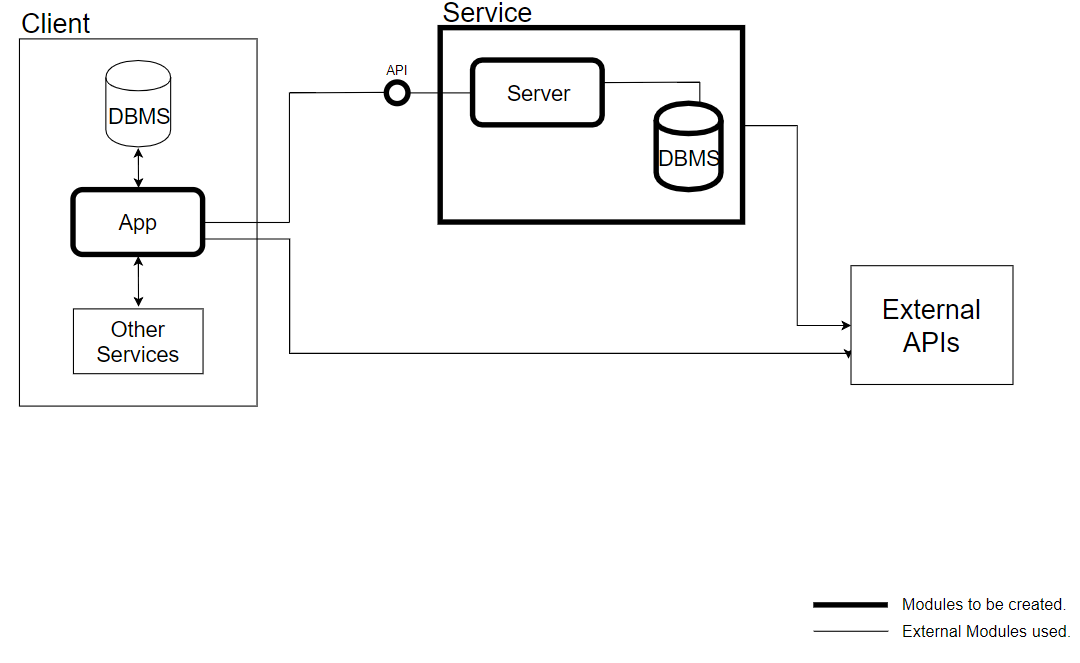
\includegraphics[width=\textwidth]{images/project-structure/system-structure.PNG}
            \caption{System structure.}
            \label{fig:systemstructure}
        \end{figure}  
        \newpage    

    \section{Client Application}
        The first step was choosing the proper technology\cite{technologiesclientdocs} for this component and Kotlin \cite{kotlinwebsite} seemed the best choice as far as supported programming languages 
        of the Android Platform go, because it introduces functional features to support interoperability and intelligibility. The main reason Kotlin was chosen was to improve the coding experience in a way that was practical, fast, and effectual.
        After the technology was decided the definition of the Client application\cite{clientapplicationdocs} Architectural principles followed, which is the core of this component. 
        So the principles were the separation of concerns, where each module has its own purpose and that the user interface(UI) 
        should be driven from a model, which in turn means that the view objects and the application components are independent of data handlers.
        
        
        \subsection*{Route Creation}
            The Route Creation functionality is already done in the Client Application and is where the user can create its own Routes to show others, when searched. 
            Initially the user is asked where is the location of the Route and then using the google maps API the map is obtained and it is zoomed to the chosen location. 
            After that, the user can click on the map to select the Route points which are then connected by the application, forming a route. When the route is completed  
            the user needs to fill a form to complete the metadata such as the name, description and category of the Route that is about to be created. 
            The Route metadata could have some improvements in the future, to be more useful when searching for the correct Route.
    
        \subsection*{Communication with the Social Routing API}
            To build communication with the Social Routing Service\cite{communicationwithexternalapis}, the library Retrofit\cite{retrofit} was used, which is responsible for making Hypertext Transfer Protocol(HTTP) \cite{httponlinedocs} requests.\par 
            \newpage

        \subsection*{Infrastructure Design}
            The infrastructure design\cite{clientdesignandimplementationdocs} of the Client Application follows the principles described before and as such, it can be divided in four blocks: Activities and Fragments, 
            View Models, Repository and the Remote Data Source. Where each has one objective in the Client Application:
        \begin{itemize}
                \item Activities and Fragments: contain logic that handles the UI and the actions related to operating system. These are the components that 
                the user can interact with and obtain feedback about what is currently happening on the application.
                \item ViewModels : when the UI experiences a change, the ViewModel calls other components to load the data, and it can forward user requests 
                to modify the data, however the ViewModel doesn't know about UI components, it is completely separated from them.
                \item Repository : handles data operations, knows where to get the data from and what API calls to make when data is updated. 
                A repository can be considered to be a mediator between different data sources, such as web services.
                \item Remote Data Source: module that has the objective of communicating with external APIs and it communicates by doing requests to some Services, 
                including the Social Routing API.
            \end{itemize}
    
        \begin{figure}[h]            
            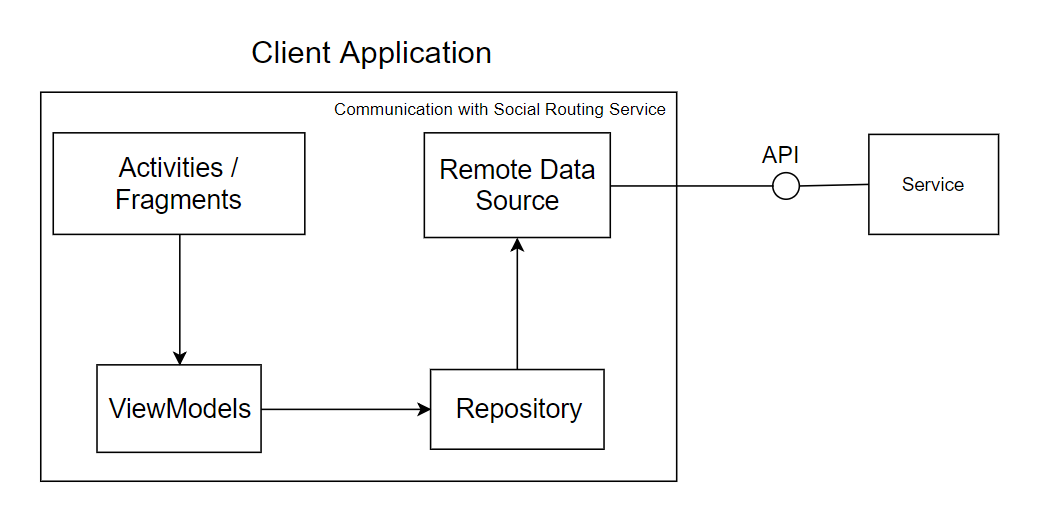
\includegraphics[width=\textwidth]{images/project-structure/social-routing-client-application-structure.PNG}
            \caption{Client Application Structure.}
            \label{fig:clientapplicationtructure}
        \end{figure}          
    
        \newpage

    \section{Social Routing Service}

        The Social Routing Service is responsible for providing access to data and functionalities to a client through an an HTTP based API. It receives HTTP made requests
        with certain specifications and responds with resources generated by the the server. The following diagram details the building blocks of the service:

        \begin{figure}[h]            
            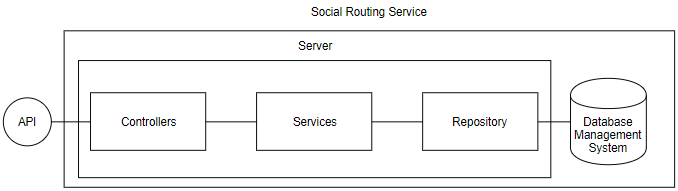
\includegraphics[width=\textwidth]{images/project-structure/service-structure.PNG}
            \caption{Social Routing Service structure.}
        \end{figure}  

        \subsection{Social Routing API}          
           
            The goal of the Social Routing API is to expose the service's functionalities to a client, in this case an Android\cite{androiddocs} based client application. The API
            should be used to store or retrieve routes and user information, as well as to find the closest route available to a specific user or location.\par
            It was built in the Kotlin programming language and uses the {Spring MVC framework} \cite{springwebsite}. The build system is that of the server,
            which they both share with the framework itself, Gradle \cite{gradlewebsite}. \par 
            All API access is done over HTTP and the API data is sent and received in the JSON \cite{jsonwebsite} format. The exception is on error responses
            which follows the JSON+problem \cite{jsonproblemonlinedocs} standard. \par
            Currently the API supports requests in a limited number of HTTP \textit{verbs} (GET, POST, PUT, DELETE) \cite{apihttpverbsdocs}, and has a functional but incomplete error handling system. 
            Some request specifications are already complete, such as the media type desired in a POST request but some are not such as user authentication. 

            \newpage

            \subsubsection*{Endpoint for Route Creation}
            The first task when building the API was to provide a way for a Route to be created because of the considerations it requires. Namely, the 
            definition of a Route and the metadata it needs in order to be stored and retrieved.\par
            
            This goal was achieved with success \cite{routecreationdocs} but with some minor problems in the definition aspect occurring from time to time. 
            Initially a route was a set of coordinate pairs, that each had the latitude and longitude of a given geographic point, but 
            as the project grew the metadata required to define a route grew with it. At this time, for a route to be created it requires not only the 
            set of coordinates but also its creator's information and its assigned categories.

            \subsubsection*{Finalization}
            After the the API's structure was complete with the creation of a route the rest of the endpoints were added and are now functioning properly \cite{apidocs}.
            There are some functionalities left that will only be complete later on, like user authentication and error handling, the last one being now done 
            but in an incomplete albeit functional way.
            When adding each of the endpoints to the API the difficulty relied in a separation of concerns and requirements of both the server side and client side modules.
        
            \newpage
        
        \subsection{Server}    
            The role of the server within the system is to receive data, transform it, and either store it or process it and return it as a response. The technologies
            it requires to function are the same as the API.\par
            The \textit{flow} of an HTTP request that arrives on the server goes through the following pipeline: a Controller is assigned to a specific endpoint which might use
            a service. If the request requires stored data the service will request it from a repository, if not, the service processes the data and returns 
            it in the correct form back to the controller which responds to the request with a response in a well defined format, depending on the request made. 

            \subsubsection*{Communication with the Database Management System}
            Initially the communication with the database was made using Spring Data JPA \cite{springjpadocs} but after the initial implementation with it, it revealed 
            itself to be time consuming on the learning side, and limited in the management of the database connection and SQL queries desired. 
            That caused a switch to a different approach, using JDBI \cite{jdbidocs} which is an API that is built on top of the JDBC driver \cite{jdbcdocs} and is used directly in 
            the server by the Repository component to communicate with the database.        

            \subsubsection*{Infrastructure Design and Implementation}
            The structure of the server follows the one showed in figure \ref{fig:systemstructure}. A controller receives HTTP requests and forwards them to a service, which in turn will process the data, and if required will
            request or store persistent data through the use of a repository.\par
            An also very important part of the server is also the conversion of data. Currently, a received request is transformed from received data in the JSON format to an input type object which is received by a controller, then to a data 
            transfer object and sent to one or multiple services and after that to a domain object which might be sent to a repository if database storage or retrieval is necessary.\par
            Setting this goal so early in the timeline allowed us to establish a foundation to build on top of in a very quick fashion, being that most of the work was done decided initially the rest 
            was just a question of adding an extra Repository, Service or Controller as well as the required type converters. 

            \subsubsection*{Remaining Functionalities Except Search}
            The functionalities of the server required in this point were all the ones considered to support a functional API and as such, after the initial structure was done, most of the requirements
            that followed were a matter of adding and extra component horizontally being that the vertical structure was already complete. As far as the search functionality goes, it is implemented in 
            a minimalistic version, allowing for route searching by location only.

            \newpage

        \subsection{Database Management System}
            The database management system chosen was PostgreSQL \cite{postgresql}, using the hybrid functionality of storing valid JSON directly in a table field \cite{postgresqljson}. The database is used to store
            all entities required for the service to function and to deliver them to repositories in need. 
            The decision of choosing JSON as a type to store data comes with the need of storing large sets of coordinates belonging to a single entity, this will allow us to 
            make faster and easier calculations of times and distances between routes and points rather than if a Point was it's own database entity. 

            The following entity diagram represents the structure of the database:
            \begin{figure}[h]            
                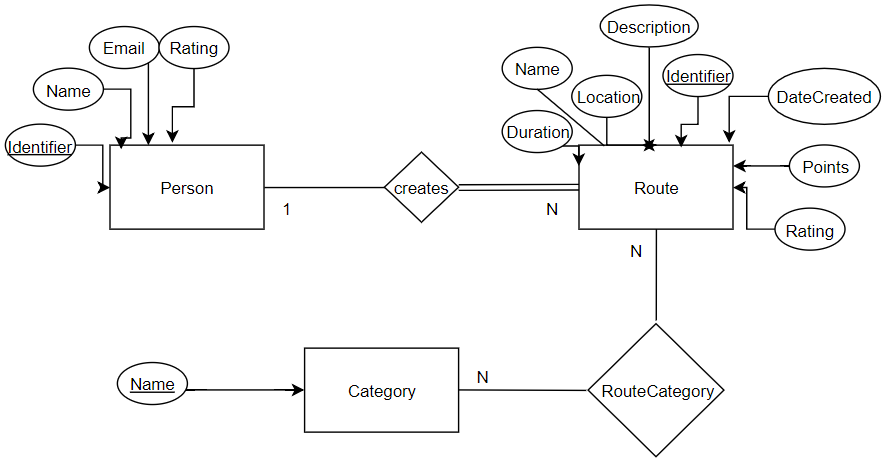
\includegraphics[width=\textwidth]{images/project-structure/dbms-structure.PNG}
                \caption{Entity Relationship Diagram.}
            \end{figure}   

            \subsubsection*{Route Saving}
            Route saving, like the first points of each other component, was chosen to be able to have a well defined structure of the whole project as quickly as 
            possible with the goals of structure first, implementations later. After defining a route the project had a fully functional minimalistic structure.

            \subsubsection*{Remaining Entities}
            After the initial structure was built the remaining entities were added to the database as needed. To maintain integrity and consistency of the data functions were added to support more complete queries that manipulate multiple tables.
            When inserting a route for example, the route has to reference at least one category, and as such an insert to the route table has to guarantee an insert to the RouteCategory table. The procedures are called by the repositories and executed by the database.

            \newpage
        
    \section{Updated Timeline}
        \begin{figure}[H]
            \begin{adjustbox}{addcode={
                \begin{minipage}{\width}}{
                    \caption{Updated timeline.}
                    \label{fig:updatedTimeline}
                \end{minipage}},rotate=90,center}
            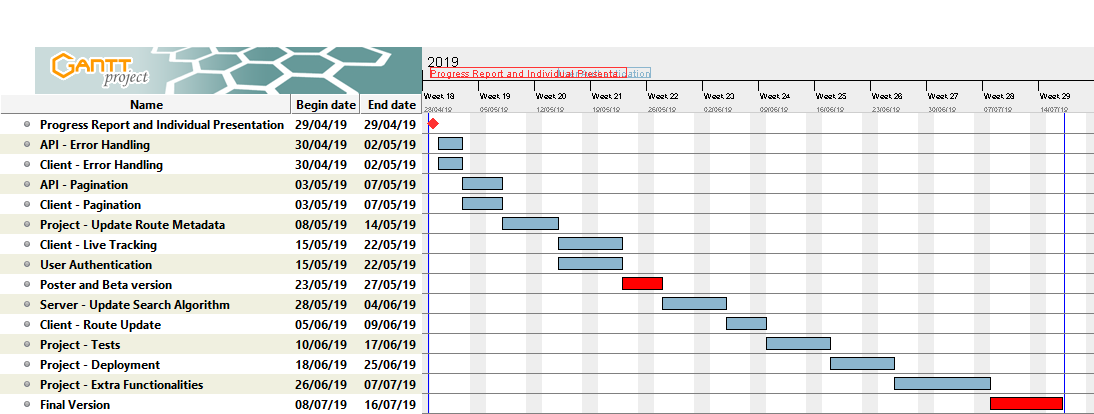
\includegraphics[width=0.9\textheight]{images/timeline/updatedTimeline.PNG}
            \end{adjustbox}
        \end{figure}
        \newpage

    \section{Risks}

        The main risk while making this project is the time to complete it and the way to minimize this is a well thought plan of action, hence the restructuring of the original timeline.
        The following list of risks will help us manage the time left as well as give us an idea of were we stand in the long term planning.

        \begin{itemize}
            \item Search Algorithm: given search parameters each user should have the best possible route suggested to him.  
            \item User authentication: using an external service and integrate it with both the client application and the Social Routing Service.
            \item Live tracking: the user should be able to follow the route in real time, on his device.
            \item External APIs comprehension and usage might take more time than initially expected.
            \item Tests: testing each component correctly might involve using external unknown libraries and the time necessary to create them might not be enough. 
        \end{itemize}
    
        \newpage    
    
    \section{Conclusion}    
        A major issue so far with the project was the incorrect planning of the first timeline. The dates for the deliverable milestones (progress report, beta and final version)
        were considered to be about one month earlier than the actual correct date and therefore the progress cannot be based solely on the original timeline. 
        However, all the goals set for before the original delivery date of the progress report were accomplished and because of the extra time, some features planned 
        only for after the delivery were also done. The tasks completed after the delivery were:\par

        \begin{itemize}
            \item Client: the route search functionality is already done, albeit in a minimalistic way. The user profile is also completed as well as route visual representation. All these tasks were in the API - finalize timeline task point.
            \item Social Routing Service: close to complete lacking only (complete) error handling, pagination and search algorithm improvement.
        \end{itemize}

        Considering this initial mistake in the original timeline creation, we created a new one to better suit the needs of the project's implementation.
        Creating a new timeline has some risks and as such we dedicated a chapter to list them.
        One of the first problems encountered was how a route should be defined. Several iterations were made before arriving at the current one. We avoid saying final
        because the definition of a route is susceptive to change when new functionalities are implemented.
        While implementing the Client Application some problems were encountered when utilizing the Google Maps API, namely the API key and the service's usage. 
        Without an account with a credit card associated we were limited to one API call per day, which was limiting our testing capabilities. This was overcome by creating a wallet (offered by the service with an initial value).
        The process that is required to create a route was also a problem, there are some considerations to be had due to the nature of a path: where it starts, where it ends, if it is circular, if it is doable in a determined time amongst others.
        This topic is intertwined with route definition, changes in the definition also change the creation.\par
 
        The Service had problems initially with the connection to the Database Management System, specifically because the choice of technologies was not the appropriate one, which
        forced a shift to a different one. This used valuable time because two different libraries were learned (Spring Data and JDBI) and later Spring Data was discarded.


        \newpage    
    
    \printbibliography



\end{document}
